\documentclass[11pt,a4paper]{article}
\usepackage[utf8]{inputenc}
\usepackage[T1]{fontenc}
\usepackage{amsmath,amssymb,amsthm}
\usepackage{graphicx}
\usepackage[margin=2.5cm]{geometry}
\usepackage{hyperref}
\usepackage{xcolor}
\usepackage{booktabs}
\usepackage{authblk}
\usepackage{cite}
\hypersetup{colorlinks=true,linkcolor=blue,citecolor=blue,urlcolor=blue}

\title{\textbf{Discrete Drainage Dynamics:\\
A Bounded, Conservative Local Rule for\\
Newtonian-Like Potentials}}
\author[1]{Stanislas Dewavrin}
\affil[1]{Independent researcher \\ \texttt{dewavrin.iphone@gmail.com}}
\date{April 2026}

\begin{document}
\maketitle

\begin{abstract}
\noindent
\textbf{Discrete Drainage Dynamics (DDD) is an analogue-substrate
programme.} It does not contest General Relativity or the
Standard Model: those are treated as the empirical anchors that
any analogue must reproduce in the appropriate continuum limit.
DDD asks the more modest, exploratory question of whether some
of the \emph{forms} that appear fundamental in current physics
can be made mechanically legible inside a deliberately simpler,
local, discrete, finite-reserve substrate. The programme is
exploratory and conditional; the present paper introduces the
substrate.

We define a deterministic, parallel, local update rule on a
discrete graph, constrained by six operational axioms (locality,
determinism, internal conservation, reserve non-negativity,
finite per-link bandwidth, large-scale isotropy). Each node
carries a non-negative reserve $R_i \ge 0$ with rest value
$R_0$; each oriented link carries a non-negative directional
flux; the rule alternates a link update and a node update with
a per-node rate-limiter $\beta_i \in [0,1]$ that prevents the
reserve from becoming negative. The flux on a link is written
in a general form involving a \emph{mobility function}
$\mu(R)$, the choice of which is left as an explicit hypothesis
of the framework (companion papers explore alternative
hypotheses). The present paper adopts the constant-mobility
hypothesis $\mu \equiv 1$ as the calibration regime in which
finite-resource non-linearity is inactive. In this regime, far
from the non-negativity floor, the rule's steady state coincides
with the discrete Poisson equation, and we measure on the
lattice that the static profile around a point source follows
a $1/r$ form with the continuum coefficient at the percent
level. We emphasise that the $1/r$ form is the \emph{expected}
analogue baseline (any 3D discrete diffusion produces it); the
contribution of this paper is the bounded-reserve, rate-limited
rule and the mobility hypothesis framing, which together
provide a finite-resource analogue substrate for the non-linear
phenomena studied in companion papers. We do not derive
Newton's $G$, GR, or any aspect of the Standard Model; we
calibrate $G$ from observation and treat the underlying
physical theories as anchors, not as targets to replace.
\end{abstract}


\noindent\fbox{\parbox{0.96\textwidth}{\small
\textbf{What this paper makes mechanically legible.}
Newtonian gravity treats finite signal-propagation speed as an
empirical input (deferred to GR's postulate of $c$) and a
plain Poisson equation has no mechanism preventing pathological
sinks. \emph{This paper} introduces a discrete substrate whose
locality (L1) and finite per-link bandwidth (L5) \emph{force}
a propagation-speed ceiling by construction, and whose
non-negativity rate-limiter (H-ratelimit) regulates would-be
singularities at the substrate level. \textbf{Leverage:} the
existence of a propagation ceiling and the regularity of
sources become \emph{consequences} of the discrete rule, not
postulates --- the ontological seed for Papers~II--IV's
mechanical readings of $g_{tt}$, $c$, and the deflection
factor of two.
}}
\bigskip


\section{Programme positioning and analogue framing}
\label{sec:framing}

Before stating the claims of this paper, we make explicit the
position the entire DDD programme takes with respect to
established physics, because misreading on this point would
collapse the rest of the work into something it does not
attempt to be.

\paragraph{What DDD is.} DDD is an analogue-substrate
programme. It explores whether some \emph{forms} that appear
fundamental in continuum physics (e.g.\ a static $1/r$
potential, a Schwarzschild-like clock-rate factor, a
Lorentz-like dispersion, gauge-like couplings) can arise as the
continuum limit of simple local update rules on a finite-reserve
discrete substrate. The programme is exploratory: it identifies
which simple substrate assumptions are sufficient to reproduce
selected continuum forms, where those analogies break down, and
whether remaining unexplained constants tie to discrete
structural features.

\paragraph{What DDD is not.} DDD does not contest General
Relativity, Newtonian gravity, or the Standard Model. Those
empirical theories are treated as anchors the analogue must
reproduce in the appropriate continuum limit; any deviation
between the analogue and the empirical theories is a falsifier
of the analogue, not of the empirical theories. The programme
does not aim to overthrow the current formalism; it aims to
make some of its most mysterious structures \emph{mechanically
readable} inside a simpler model. We use phrases such as
``recover the form of'', ``reproduce the analogue of'',
``substrate-internal derivation'' rather than ``derive''
unconditionally; bare statements of the form ``we derive
[law of physics]'' are out of scope and never claimed.

\paragraph{Empirical anchors and falsifiability.} Throughout the
series, GR and the SM provide the empirical anchors. The
analogue is held to the standard of (i) reproducing the
appropriate continuum form within a stated regime of validity,
(ii) being explicit about where it breaks down (UV
corrections, finite-size effects, scope limits), and (iii) being
falsifiable by precision tests of the relevant continuum
prediction. The reader should regard each ``derivation'' in
this and subsequent papers as internal to the analogue,
conditional on stated hypotheses, and matched against the
empirical anchor as a consistency check rather than a
fundamental claim.

\paragraph{Which mystery does this paper address?}
Per the targeted mystery list of the DDD programme
(SERIES\_FEEDBACK §0.bis), this paper contributes to two
\emph{why}-questions, in foundational form:

\begin{itemize}
\item \textbf{Mystery~\#1 (the speed-of-light ceiling).} The
finite per-link bandwidth $\alpha$ and the discrete tick $\tau$
together produce a propagation-speed ceiling $\sim \alpha\,\ell$
in the analogue. The present paper does not yet identify this
with the empirical value of $c$; that identification awaits
Paper~III's Floquet sector.
\item \textbf{Mystery~\#2 (gravitational potentials).} The
constant-mobility baseline reproduces the form of Newton's
$1/r$ as the analogue's weak-field static limit. The present
paper does not address why the analogue's coefficient matches
the empirical value of $G$; that calibration is the subject
of Paper~II.
\end{itemize}

The contribution is incremental: this paper supplies the
analogue substrate within which subsequent papers address the
quantitative *why*-questions for $c$, $G$, gravitational time
dilation, kinematic time dilation, etc.

\paragraph{Distinctive contribution and ontological reading.}
The $1/r$ form is not novel as a mathematical result --- any 3D
discrete diffusion produces it, and Newtonian gravity describes
it precisely. The contribution of this paper is therefore
\emph{not} the $1/r$ law itself but the substrate
\emph{ontology} from which it arises and the structural
features that distinguish a finite-bandwidth lattice rule from
a plain continuum diffusion. Three distinctive ingredients are
introduced, each absent or implicit in the standard treatment:

\begin{enumerate}
\item \textbf{Finite per-link bandwidth.} The propagation
coefficient $\alpha$ is a structural rate, not a free
phenomenological parameter; it caps how fast information can
move on the substrate. Standard Newtonian gravity has no
mechanical statement of \emph{why} signals propagate at finite
speed at all (this question is deferred to GR's postulate of
$c$, which itself is an empirical input). DDD's locality axiom
forces a propagation-speed ceiling $\sim \alpha\,\ell$
\emph{by construction}, before any identification with $c$.
This is the foundational ingredient that Paper~III uses to
read the speed-of-light ceiling as a substrate consequence.

\item \textbf{Reserve non-negativity floor and the
rate-limiter (H-ratelimit).} The discrete rate-limiter
$\beta_i \in [0, 1]$ enforces $R_i \ge 0$ at the substrate
level. In the continuum analogue, this floor would not exist:
a plain Poisson equation has no mechanism preventing
unbounded sinks or pathological singularities. Here, the
rate-limiter is a structural regulator that anticipates the
\emph{singularity-resolution} programme of Paper~II: where GR
predicts a curvature singularity at $r = 0$ (the marker of the
continuum theory's limit), the discrete substrate has a
non-negativity floor that activates before the analogue's
$R \to 0$ horizon and prevents the pathological divergence.

\item \textbf{Two-step bipartite alternation (H-step-order).}
The Link/Node alternation is locally causal by construction:
each sub-step reads a fixed neighbouring state and writes the
corresponding update, with no self-reference within a tick. In
the continuum, causality is imposed via Lorentzian metric
structure post-hoc; here it is built into the substrate's
update topology from the outset.
\end{enumerate}

\paragraph{Why this matters for the rest of the series.}
The substrate ontology of this paper is the foundation on
which all subsequent papers stand. Paper~II uses the
finite-reserve floor to read Schwarzschild $g_{tt}$ as
bandwidth throttling \emph{and} to begin regularising the BH
singularity. Paper~III uses the finite per-tick bandwidth to
read $c$ as a substrate consequence rather than an ad-hoc
postulate. Paper~IV uses the same bandwidth profile to derive
the weak-field deflection coefficient. None of these moves
would be possible in a continuum theory without the discrete
substrate's structural ingredients (i)--(iii). The present
paper is not a result paper: it is the \emph{ontological seed}
the rest of the series grows from.



\section{Foundational principles of the analogue substrate}
\label{sec:principles}

We constrain the substrate by six operational axioms. They are
operational in the sense that each is a statement about what
the local update rule may or may not depend on, not a statement
about deeper physics.

\begin{enumerate}
\item[(L1)] \textbf{Locality.} Every elementary update reads
only a node and its immediate neighbours through incident
links. There is no action at a distance within a tick.
\item[(L2)] \textbf{Determinism.} The rule is fully specified by
the current substrate state; no randomness or hidden variables
enter the elementary update.
\item[(L3)] \textbf{Internal conservation.} Inter-node flux
exchange preserves total reserve exactly. External sinks (e.g.\
a point source) enter as explicit bookkeeping at the boundary,
not as an internal violation.
\item[(L4)] \textbf{Reserve non-negativity floor.} The reserve
satisfies $R_i \ge 0$ at all times: a node cannot push reserve
it does not have. A per-node rate-limiter
$\beta_i \in [0,1]$ (Eq.~\eqref{eq:beta} below) enforces this
without flux clipping at the link level.
\item[(L5)] \textbf{Finite per-link bandwidth.} Outgoing flux
on a link is bounded; propagation is time-stepped, not
instantaneous. The basic propagation coefficient $\alpha$ has
the dimensions of a rate.
\item[(L6)] \textbf{Large-scale isotropy.} The continuum limit
of the rule is rotationally symmetric. We work on regular
graphs (cubic, BCC) of degree $\ge 6$ on which this is realised.
\end{enumerate}

\paragraph{The structural question grid (front-loaded).}
The DDD analogue is built up progressively across the paper
series: Paper~I states the substrate foundations, but later
papers extend into sectors (gauge, spinor, cosmogenesis) that
are not addressable here without first introducing the
appropriate substrate ingredients. To make this trajectory
visible from the foundations \emph{and} to defuse the
appearance of post-hoc accretion (cf.\ SERIES\_FEEDBACK §5),
we list the structural questions the entire series must
answer, and indicate which paper occupies each slot:

\begin{description}
\item[Q1 --- Composition.] What primitive degrees of freedom
sit on nodes? On links? Paper~I introduces the scalar reserve
$R_i$ on nodes and the directional flux $F_{i\to j}$ on links
(this paper). Paper~III extends nodes with the spinor $\psi_i$
and links with the diagonal twist phase. Paper~VI extends
links with the U(1) orientation phases $\psi_{ij}$ and nodes
with orientations $\alpha_i$.

\item[Q2 --- Update rule.] How does the substrate state
evolve in one tick? Paper~I introduces the bipartite Link/Node
alternation with constant mobility (this paper). Paper~II
extends to source-side bandwidth-throttled mobility
$\mu(R) = R/R_0$. Paper~III extends to the Floquet two-step
$U_F = U_B U_A$ for the spinor sector. Paper~VIII extends with
a temporary autocatalytic source term during the cosmogenetic
creation epoch.

\item[Q3 --- Topology.] What graph carries the substrate?
Paper~I uses regular cubic and BCC lattices (this paper). The
unit-cube combinatorics is used in Paper~VI (body-diagonal
Wilson loop) and Paper~VII (cube-surface Wilson surface). No
paper to date relaxes the regularity or local connectivity.

\item[Q4 --- Number of distinguishable readable fields.]
How many independent local quantities are exposed by the
substrate? Paper~I exposes the scalar reserve $R_i$ alone.
Paper~III adds the two complex amplitudes of the spinor
$\psi_i$. Paper~VI adds the U(1) orientation phase. The
substrate's local degrees of freedom grow only when a new
sector is opened.

\item[Q5 --- History / frame structure.] What history of past
states does the rule depend on? Paper~I's rule is first-order
in time (depends only on the previous tick). Paper~III's
Floquet two-step requires sub-tick decomposition (alternation
between two half-steps within one tick). Paper~VIII's
cosmogenetic regime depends on the global epoch indicator
$t < t_s$ vs $t \ge t_s$. No paper requires a non-local
historical dependence that would violate (L1).

\item[Q6 --- Hypotheses needed to close each sector.] Each
sector requires a labelled hypothesis (per
SERIES\_FEEDBACK §0.ter) to close at the metric/observable
level. Paper~I introduces (H-mobility), (H-const),
(H-step-order), (H-ratelimit) for the foundational sector.
Subsequent papers add: (H1) additivity, (H2) bandwidth
identification (Paper~II); (F-twist) topological winding
(Paper~III); (H-spatial) photon coupling (Paper~IV);
(H-feedback) self-consistent back-reaction (Paper~V);
(H-orient) orientation-energy functional (Paper~VI);
(H-shared-prefactor) (Paper~VII); (H-autocatalysis) +
(H-cosmogenesis) (Paper~VIII). The cumulative cross-paper
ledger is in \texttt{EPISTEMIC\_SPINE.md} at the series root.
\end{description}

\noindent\emph{Why front-load this grid.} Without this grid,
each new paper looks like an additional structural ingredient
introduced \emph{ad hoc}. With the grid, each new paper
visibly fills a slot that was already named here. This is the
distinction between \emph{scope-extension} (legitimate
progressive disclosure) and \emph{post-hoc accretion}
(modification of an earlier sector under data pressure)
formalised in SERIES\_FEEDBACK §5.

\paragraph{Class constrained by (L1)--(L6).}
Within (L1)--(L6), the admissible local rules form a class of
two-step bipartite alternations (link-then-node updates) on
regular lattices with a per-node rate-limiter; we adopt the
minimal linear-flux representative described in
Sec.~\ref{sec:rule}. The bipartite-alternation structure is not
\emph{forced} by (L1)--(L6) alone --- a fully synchronous update
is not strictly excluded, but it would require a precedence
convention that effectively reintroduces an alternation; we
adopt the explicit two-step form for clarity and to match
Paper~III's stateful-link extension.

\paragraph{Hypothesis (H-mobility): the mobility function is a
structural choice.}
Within the (L1)--(L6) class, the form of the mobility function
$\mu(R)$ is not uniquely determined: the axioms admit a family
of source-side modulations parameterised by $\mu$. We therefore
declare $\mu(R)$ a \emph{hypothesis} of the framework, not a
derivation:

\begin{description}
\item[(H-mobility)] The directional flux on a link is modulated
by a non-negative mobility function $\mu(R)$ of the source
node's reserve, normalised so that $\mu(R_0) = 1$ at rest. The
choice of $\mu$ is a structural hypothesis whose microscopic
origin is not addressed in this paper; companion papers
(notably Paper~II) study alternative choices.
\end{description}

\paragraph{Hypothesis (H-const): constant-mobility baseline.}
The present paper adopts:

\begin{description}
\item[(H-const)] $\mu(R) \equiv 1$. This models a regime in
which source-side bandwidth throttling is inactive. It is the
\emph{calibration regime} in which the rule reduces, in the
linearised continuum limit, to the discrete Poisson equation
and recovers the analogue $1/r$ baseline. (H-const) is a
sub-hypothesis of (H-mobility); alternative choices, such as
$\mu(R) = R/R_0$ studied in Paper~II, define qualitatively
different non-linear regimes.
\end{description}

The rule, the rate-limiter, and the linearised-continuum
analysis below are therefore conditional on (L1)--(L6) +
(H-mobility) + (H-const). The microscopic origin of (H-mobility)
is the principal open problem of the analogue framework
(Sec.~\ref{sec:open}).

\section{Main claims and scope}
\label{sec:claims}

We make three claims.

\begin{enumerate}
\item We define a deterministic, parallel, two-step local rule
on a discrete graph. The reserve is bounded below by zero
($R_i \ge 0$, the physical floor: one cannot drain what is not
there); $R_0$ is the rest value, but the reserve is free to
exceed it in excited regimes treated in companion papers. The
flux on a link involves a mobility function $\mu(R)$ that we
leave as a structural choice of the framework; the present
paper studies the constant-mobility baseline $\mu \equiv 1$.
\item Run as a stationary linearised simulation with a point
source on a cubic lattice, the rule (with $\mu \equiv 1$)
produces a radial profile compatible with $1/r$ in the bulk,
with a coefficient that matches the discrete continuum
prediction at the percent level across $L \in \{64, 128, 160\}$.
\item The internal flux-exchange rule preserves total reserve
exactly. Non-negativity of the reserve is enforced by
rate-limiting the outgoing fluxes and external sinks of a node
in proportion, so that emission stops when the reserve reaches
zero; no mass is created or destroyed by the internal rule.
This is the structural feature that distinguishes the rule
from a plain discrete heat equation.
\end{enumerate}

\paragraph{What we do \emph{not} claim (defensive
restatement).} The constant-mobility analogue baseline of this
paper is not a claim about fundamental physics. We do not
derive Newton's gravitational constant in physical units; we
calibrate it against the observed value. We do not derive
General Relativity, the Newtonian limit of GR as a fundamental
law, or any property of the Standard Model: those theories are
empirical anchors, treated outside the analogue. We do not
show that the rule is unique.
We do not derive the mobility function $\mu(R)$; the
constant-mobility baseline of this paper is a choice within a
family of possibilities. We do not assert that the $1/r$
result is itself novel: it is not. What is novel is the rule,
the mobility framing, and the structural features (reserve
non-negativity, rest level $R_0$, two-step alternation,
rate-limited fluxes) that make the rule non-trivial in the
regimes explored in the companion papers.

\subsection*{Motivation and significance}
\addcontentsline{toc}{subsection}{Motivation and significance}

The purpose of this paper is \emph{not} to rediscover the
$1/r$ potential. Any linear diffusion or graph-Laplacian model
in three dimensions has a Green function with this behaviour.
The purpose is instead to define a local, conservative substrate
rule whose weak-field limit reduces to the discrete Poisson
equation, while retaining \emph{finite-resource} structure
outside that limit.

This distinction matters for the rest of the DDD programme. A
plain heat equation can reproduce $1/r$, but it has no physical
floor, no finite local budget, no source-side mobility, and no
natural saturation regime. The rule introduced here adds these
ingredients: every node carries a non-negative reserve $R \geq
0$, every outgoing flux is rate-limited by the available local
budget, and the mobility $\mu(R)$ controls how the source
node's reserve modulates emission. These are the substrate
features on which the companion papers depend.

The baseline $\mu \equiv 1$ studied in this paper is therefore
a \emph{calibration and validation regime}. It verifies that the
rule reduces to the expected Poisson behaviour when the
finite-resource constraint is inactive. The non-trivial physics
begins when $\mu(R) \neq 1$ (Paper~II's clock-rate suppression
and Schwarzschild geometry), or when the reserve floor $R = 0$
becomes active (saturation, horizon-like bandwidth limit), or
when the spinor and gauge-sector back-reactions of Papers~III,
VI, and VII activate. Paper~I supplies the conservative local
substrate on which they all depend.

A diagnostic of this finite-resource structure is that
superposition of source profiles, exact in the linear regime,
must \emph{break down locally} when the reserve floor or the
mobility nonlinearity becomes active. We exhibit this directly
in \S\ref{sec:two-source} as a sanity check.

\section{Physical picture in plain words}
\label{sec:picture}

Imagine a fine three-dimensional grid. At each grid point sits
a reservoir holding a non-negative amount of stuff. There is a
rest level $R_0$ that the reservoirs all sit at when the system
is undisturbed; reservoirs can be excited above $R_0$ or
drained below it, but they cannot go below zero. Between
neighbours run pipes that carry a non-negative flow of stuff
from the fuller reservoir to the emptier one, at a rate
proportional to the level difference, optionally modulated by
how much stuff the source actually holds. A reservoir cannot
deliver more stuff than it actually has: a node at zero stops
emitting.

If we start the system at the rest level $R_0$ everywhere,
drain one point, and let the system settle, the bulk reservoir
levels relax into a stationary pattern. With the simplest
choice of mobility ($\mu \equiv 1$, the case of this paper),
far from the source the pattern reduces to the textbook
discrete Poisson solution and the deficit $R_0 - R_i$ falls as
$1/r$ with distance. Other choices of mobility yield
qualitatively different non-linear regimes, studied in
companion papers.

The interesting cases are where the floor matters. Near a
strong drainage point, the reservoir level can be driven to
zero, and emission from that node stops. In this regime the
rule is no longer a discrete heat equation: it is a non-linear
update with a finite-resource bound. The companion papers
explore those regimes (Schwarzschild-form behaviour in
Paper~II, Floquet spinor sector in Paper~III, gauge sector in
Paper~VI, gravity-gauge coupling in Paper~VII). The present
paper is restricted to the linearised regime with
$\mu \equiv 1$, where the rule reproduces $1/r$.

\section{The substrate}
\label{sec:substrate}

\subsection{Graph and variables}

The substrate is a graph $G = (V, E)$ in which every node has
at least six neighbours and the connectivity is statistically
isotropic at large scale. We do not specify the exact topology;
in our simulations we use a regular cubic lattice for clarity,
and we have verified that BCC gives the same large-scale
spectral dimension.

For the purposes of this paper, each node $i \in V$ carries a
non-negative reserve $R_i \ge 0$, with rest value $R_0$ at
equilibrium. Each oriented link $(i, j) \in E$ carries a pair
of non-negative directional reserve fluxes $F_{i \to j} \ge 0$
and $F_{j \to i} \ge 0$. These are the only variables that
enter the linearised gravitational simulation reported here.
The non-negativity $R_i \ge 0$ is the physical floor (one
cannot drain what is not there).

\subsection*{Variables of the wider rule}

The full rule, as used in the companion papers, also assigns
to each node two angular quadratures $(T_i, I_i)$ subject to a
local coherence bound $T_i^2 + I_i^2 \le R_i$, and to each
oriented link a phase $\psi_{ij} \in [-\pi, \pi)$ with
$\psi_{ji} = -\psi_{ij}$. These additional variables drive the
gauge sector (Papers~V--VI), couple to the reserve through the
coherence bound, and do not enter the static linearised
gravitational regime treated below.

\subsection{Parameters}

\begin{table}[h]
\centering
\begin{tabular}{lll}
\toprule
Parameter & Role & Used in this paper\\
\midrule
$\kappa$    & drainage coefficient            & yes\\
$\alpha$    & flux propagation coefficient    & yes\\
$R_0$       & reserve rest value (equilibrium) & yes\\
$\mu(R)$    & mobility function (structural choice) & yes ($\mu \equiv 1$)\\
$J$         & link relaxation coupling        & no (gauge sector, deferred)\\
\bottomrule
\end{tabular}
\caption{Parameters of the local rule. The reserve floor at
$0$ is not a parameter: it is the physical statement that one
cannot drain what is not there. $R_0$ is the rest level at
equilibrium, not an absolute ceiling: the reserve can exceed
$R_0$ in excited regimes treated in the companion papers. The
mobility $\mu(R)$ is a structural choice of the framework: this
paper uses $\mu \equiv 1$, companion papers (notably Paper~II)
use other choices.}
\label{tab:params}
\end{table}

\section{The two-step tick}
\label{sec:tick}

\subsection*{Motivation}

The class of rules considered here is motivated by an old line
of inquiry on whether physics admits a microscopic
deterministic, local, iterative description --- a
``computational substrate'' in the sense of Zuse, Fredkin,
't~Hooft, Wolfram, and Lloyd
\cite{zuse1969,fredkin1990,thooft2016,wolfram2002,lloyd2006}.
We do not commit to the strong form of this hypothesis. We
adopt it as a working stance.

\subsection*{The rule}

The rule decomposes into two alternating half-steps, which we
call \emph{Link Update} and \emph{Node Update}. The bipartite
alternation is not strictly forced by axioms (L1)--(L6) alone:
a synchronous single-step update on stateless links would also
satisfy them. We therefore declare it a structural hypothesis:

\begin{description}
\item[(H-step-order)] The rule is bipartite, with Link Update
preceding Node Update within each tick. The bipartite structure
is motivated by (i) any synchronous update that simultaneously
reads and writes a node and its incident links requiring a
precedence convention logically equivalent to the alternation;
(ii) the bipartite form preserving locality (L1) and avoiding
self-reference within a tick by construction; and (iii) the
match with the stateful-link extension of Paper~III, where the
alternation becomes \emph{necessary} because the link variables
are dynamical. The Link-then-Node ordering (rather than the
reverse) is a convention; the reverse ordering would also
satisfy (L1)--(L6) and lead to a related class of rules.
(H-step-order) is therefore conditional on the same operational
considerations as (H-mobility); its microscopic origin is not
addressed here.
\end{description}

\paragraph{Constraint-class argument for the two-step
bipartite alternation.}
Within axioms (L1)--(L6), we can be more precise about
\emph{why} the two-step bipartite alternation is the canonical
representative of the rule class:

\begin{enumerate}
\item By (L1) locality, an elementary update at node $i$ depends
only on $\{R_i, R_{j \in N(i)}\}$ and the incident link states.
\item By (L2) determinism, the update is a fixed function of
its inputs.
\item By (L3) conservation, the per-tick update preserves
$\sum_i R_i$ exactly (modulo external sinks).
\item Any update that simultaneously reads and writes a node
$i$ and its incident link $(i,j)$ in the same elementary step
requires a precedence convention to resolve which value feeds
which. Adopting that convention is logically equivalent to
splitting the elementary step into two halves --- one that
reads the link state into the node, one that reads the node
state into the link. This is exactly the bipartite
alternation.
\item Conversely, any non-alternating decomposition either
allows a freshly-rewritten variable to feed the same step
(violating no-self-reference within the step) or duplicates
state by buffering both old and new values (the alternation
in disguise).
\end{enumerate}

\noindent The two-step structure is therefore the
\emph{minimal non-trivial sequentially-causal decomposition}
compatible with (L1)--(L3) on a graph where both nodes and
links carry independent state. The Link-then-Node ordering
(rather than Node-then-Link) is the only convention not fixed
by the axioms, and is the residual content of (H-step-order).
This argument generalises to Paper~III's stateful-link
extension where the alternation becomes \emph{necessary}
because link variables are dynamical.

\begin{description}
\item[(remaining open)] None of (L1)--(L6) require the rule
to be \emph{first-order} in time on the scalar reserve sector;
that further property is what enforces the diffusive
character of Paper~I's $\mu \equiv 1$ baseline. Future Floquet
or oscillator extensions (Paper~III's spinor sector) relax
that first-order property at the spinor locus only.
\end{description}

\subsection{Link Update}

During the first half-tick, the node reserves are frozen. For
each oriented link $(i, j)$, in parallel, we compute a desired
flux. We write the desired flux in the general form
\begin{equation}
F_{i \to j}^{\rm des} \;=\; \alpha\, \mu(R_i)\, (R_i - R_j)_+,
\label{eq:fluxdes}
\end{equation}
where $\mu(R)$ is a non-negative \emph{mobility function}
encoding how the available reserve at the source node limits
its ability to push reserve into a neighbour. We normalise
$\mu(R_0) = 1$ at the rest level, so that $\alpha$ retains its
meaning as the rated propagation coefficient when the source
is at rest. We do not derive $\mu(R)$ from a deeper principle;
it is a structural choice of the rule.

\paragraph{Constant-mobility baseline of this paper
((H-const), Sec.~\ref{sec:principles}).} The
present paper adopts the constant-mobility hypothesis,
\begin{equation}
\mu(R) \;\equiv\; 1,
\label{eq:mu_const}
\end{equation}
for which Eq.~\eqref{eq:fluxdes} reduces to the textbook
discrete-diffusion form
$F_{i \to j}^{\rm des} = \alpha (R_i - R_j)_+$, and the
linearised steady state is the discrete Poisson equation,
giving the $1/r$ profile measured in Sec.~\ref{sec:sim}.

\paragraph{Other mobility choices in companion papers.} The
reserve-proportional mobility $\mu(R) = R/R_0$, motivated by
local bandwidth limitation at the source node, is studied in
Paper~II, where it is shown to produce $\nabla^2(R^2) = 0$ in
the continuum limit and a profile of Schwarzschild form. Other
mobility prescriptions may be explored in subsequent papers.
Within Paper~I, none of these is invoked.

The two directions of a link are independent. Each node then
computes a rate-limiting factor that ensures the reserve stays
non-negative on its outgoing side. Define
\begin{equation}
A_i \;=\; R_i \,+\, \tau\, S_i^{\rm in},
\quad
S_i^{\rm in} = \sum_j F_{j \to i}^{\rm des},
\quad
D_i \;=\; \tau\, O_i^{\rm des} + \tau\, \kappa\, E_i,
\quad
O_i^{\rm des} = \sum_j F_{i \to j}^{\rm des}.
\label{eq:budgets}
\end{equation}
The rate-limiter is
\begin{equation}
\beta_i \;=\;
\begin{cases}
1, & D_i = 0,\\[2pt]
\min\!\left(1,\; A_i / D_i \right), & D_i > 0,
\end{cases}
\label{eq:beta}
\end{equation}

\paragraph{(H-ratelimit) Per-node balanced rate-limiter as
minimal enforcer of (L4).}
Equation~\eqref{eq:beta} is not the unique enforcement of the
non-negativity floor (L4): one could instead clip individual
link fluxes, use an adaptive sub-tick step, or apply a
softening function. We adopt the per-node balanced choice as a
structural hypothesis because (i) it scales \emph{all} outflows
and external sinks at node $i$ identically, preserving the
proportion of demand met; (ii) it activates only when demand
exceeds available reserve, leaving the rule untouched in the
linear regime; and (iii) it is the minimal enforcement
compatible with internal conservation (L3). Alternatives are
not explored in this paper; (H-ratelimit) is on the same
logical footing as (H-mobility) and (H-step-order).

The rate-limiter is applied identically to outflows and sink:
\begin{equation}
F_{i \to j} \;=\; \beta_i\, F_{i \to j}^{\rm des},
\qquad
E_i^{\rm real} \;=\; \beta_i\, E_i.
\label{eq:flux}
\end{equation}

\subsection{Node Update}

During the second half-tick, the link fluxes are frozen.
\begin{equation}
R_i \;\leftarrow\; R_i + \tau\, S_i^{\rm in}
\,-\, \beta_i\, \tau\, O_i^{\rm des}
\,-\, \beta_i\, \tau\, \kappa\, E_i.
\label{eq:nodeR}
\end{equation}
By construction of $\beta_i$, this update keeps $R_i$
non-negative at every tick.

\section{Conservation}
\label{sec:conservation}

\textbf{Total reserve, exactly conserved by internal exchange.}
The realised fluxes enter the Node Update of $j$ as
$+\beta_i F_{i \to j}^{\rm des}$ and the Node Update of $i$ as
$-\beta_i F_{i \to j}^{\rm des}$. Summed over the graph,
$\sum_i R_i$ is exactly conserved by inter-node flux dynamics.
The rate-limiter scales outflows and the local sink in the
same proportion.

\textbf{External sinks as bookkeeping.} The total reserve in
the network changes only by $\sum_i E_i^{\rm real}$. The
closed system network-plus-external-sink is conservative; the
network alone is open.

\section{Simulation: from rule to $1/r$}
\label{sec:sim}

\subsection{Derivation of the Poisson limit (constant mobility)}

We work in the constant-mobility baseline $\mu \equiv 1$. In
the linear regime $\beta_i = 1$, the two directional fluxes
satisfy $F_{i \to j} - F_{j \to i} = \alpha (R_i - R_j)$, so
$S_i = \alpha \Delta R_i$ where $\Delta$ is the discrete graph
Laplacian. In stationary regime,
$\alpha \Delta R_i = \kappa E_i$. Switching to the deficit
$\delta_i = R_0 - R_i$:
\begin{equation}
-\Delta\, \delta_i \;=\; M\, \delta_{\rm Kr}(i, i_0),
\qquad M \;=\; \frac{\kappa E_0}{\alpha}.
\label{eq:poisson}
\end{equation}
The continuum solution is $\delta(r) = M/(4\pi r)$.

\subsection{Numerical check}

\begin{table}[h]
\centering
\begin{tabular}{lllll}
\toprule
$L$ & $A_{\rm fit}$ & relative bias & statistical precision &
$N_{\rm iter}$\\
\midrule
64  & 0.07878 & $-1.01\%$ & $7.0 \times 10^{-5}$ & 5\,000\\
128 & 0.07866 & $-1.16\%$ & $5.7 \times 10^{-6}$ & 10\,000\\
160 & 0.07886 & $-0.90\%$ & $3.7 \times 10^{-6}$ & 30\,000\\
\midrule
\multicolumn{2}{l}{$A_{\rm continuum} = M/(4\pi)$} & $0.07958$ & & \\
\bottomrule
\end{tabular}
\caption{Newton-fit coefficients on cubic lattices, $M = 1$,
Dirichlet boundary, with $\mu \equiv 1$. The bias is roughly
$L$-independent at the percent level (Madelung correction).}
\label{tab:gres}
\end{table}

\subsection{Robustness: spectral dimension}

\begin{table}[h]
\centering
\begin{tabular}{lll}
\toprule
$L$ & cubic ($d_s - 3$ minimum) & BCC ($d_s - 3$ minimum)\\
\midrule
32  & 0.129 & 0.107\\
64  & 0.054 & 0.045\\
128 & 0.023 & 0.019\\
\bottomrule
\end{tabular}
\caption{Spectral-dimension residual converges to $0$ in the
IR limit on both substrates. Newtonian gravity recovered. This convergence validates the large-scale isotropy axiom (L6).}
\label{tab:dscomp}
\end{table}

\subsection{Two-source superposition and onset of finite-resource effects}
\label{sec:two-source}

As a second sanity check that distinguishes the DDD rule from a
plain graph-Laplacian, we place two identical point sinks at
separation $d = 8$ lattice spacings and compare the steady-state
deficit field $\delta_{12}$ with the linear superposition
$\delta_1 + \delta_2$ obtained from two independent one-source
runs.

\textbf{Linear regime ($\mu = 1$, weak sinks).} For sink
strength $0.001$, the reserve floor is never approached
($R_{\min} \simeq R_0 - \mathcal{O}(10^{-4})$, with
$R_{\min}/R_0 > 0.999$ everywhere), the rate-limiter
$\beta_i \equiv 1$ throughout, and the rule reduces to the
discrete Poisson equation. The relative residual
$\max|\delta_{12} - (\delta_1 + \delta_2)| / \max\delta_{12}$
is $5.4 \times 10^{-3}$, attributable entirely to lattice and
boundary truncation. Superposition holds.

\textbf{Saturating regime (rate-limiter active).} For sink
strength $12$, the reserve at each source is driven down to the
floor $R = 0$. The rate-limiter
$\beta_i = \min(1, A_i/D_i)$ (where $A_i$ is the available
reserve and $D_i$ is the demand from outgoing fluxes plus
external sinks at node $i$) drops below $1$ at depleted nodes,
capping the outgoing flux, and the steady-state field no longer
obeys superposition: the relative residual rises to
$2.7 \times 10^{-2}$, an order of magnitude above the
lattice-error baseline, and is concentrated near the saturated
sources where $\delta_1$ and $\delta_2$ would otherwise have
added linearly.

This contrast --- $\sim 0.5\%$ residual when the floor is
inactive vs $\sim 3\%$ when it is active --- is the diagnostic
signature of finite-resource physics that motivates the rule.
The deviation is not a numerical defect; it is the substrate
correctly refusing to deliver more flux than its local reserve
permits. Figure~\ref{fig:two-source} displays the central
slice of both regimes side-by-side.

\begin{figure}[h]
\centering
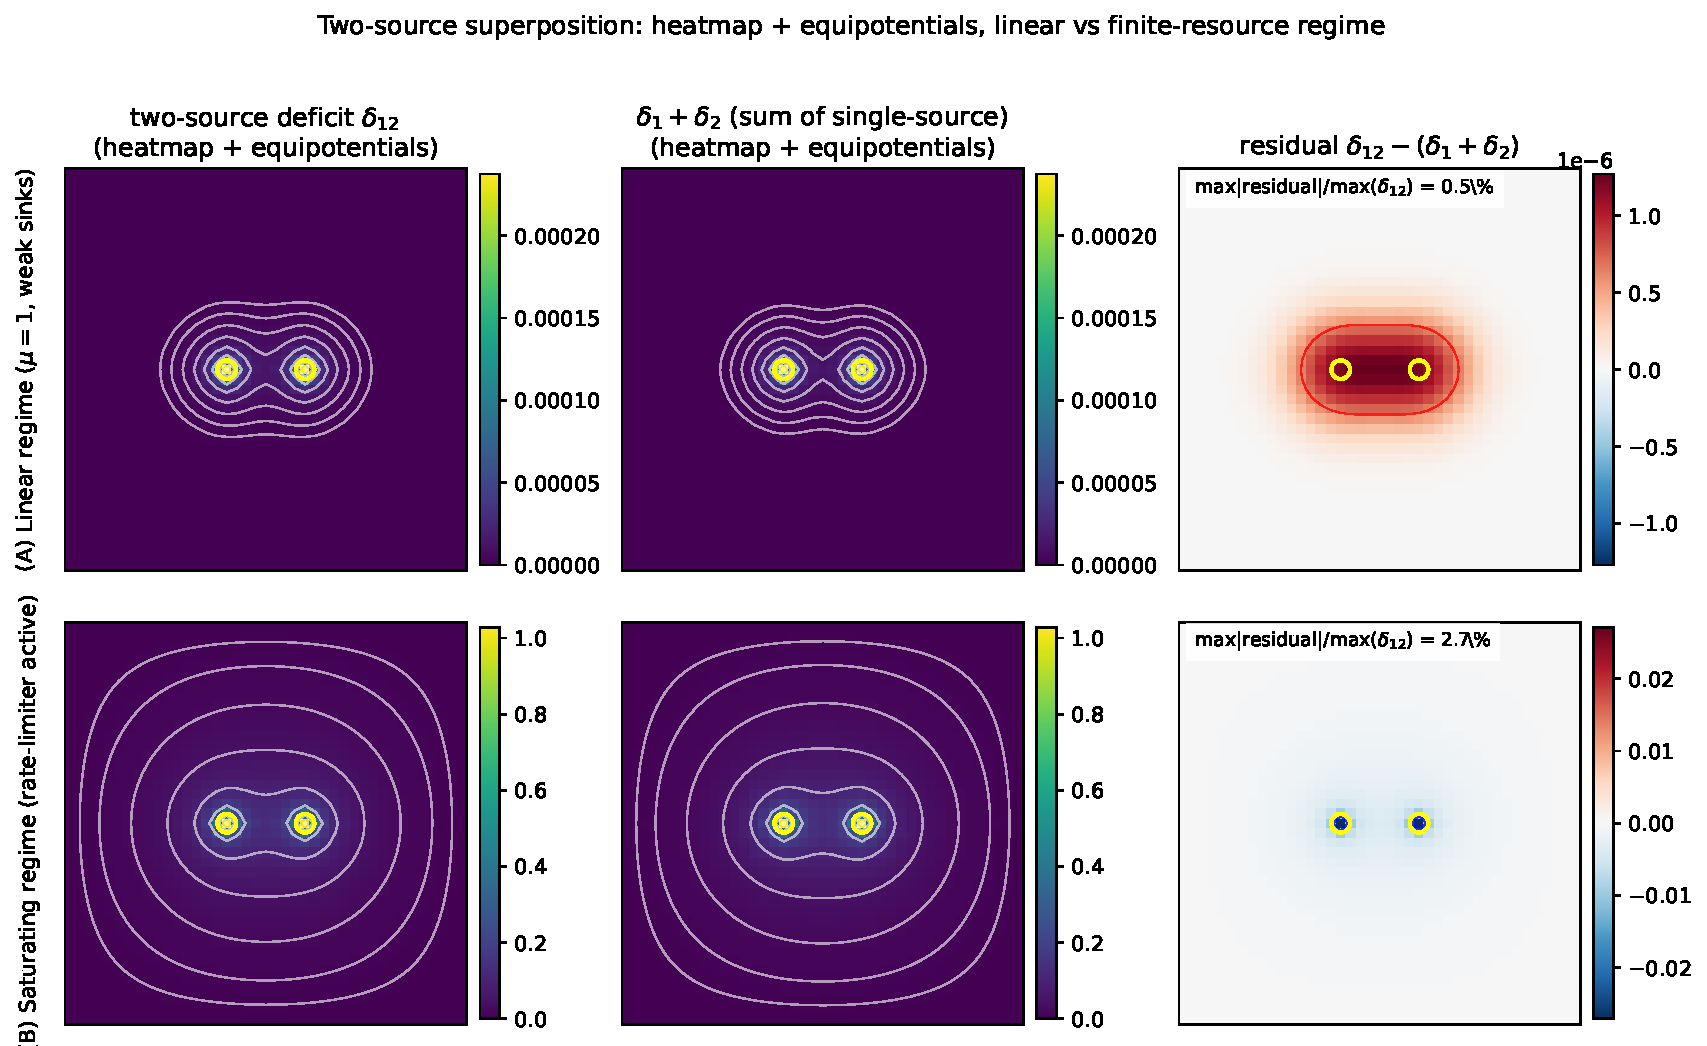
\includegraphics[width=0.98\textwidth]{figures/fig11_two_source.pdf}
\caption{Two-source superposition test. \textbf{Top row (A)},
linear regime ($\mu = 1$, weak sinks): the two-source deficit
$\delta_{12}$ (left), the superposition $\delta_1 + \delta_2$
(centre), and the residual (right). The residual is at the
$0.5\%$ level and consists entirely of lattice/boundary error.
\textbf{Bottom row (B)}, saturating regime (rate-limiter
active): the residual rises to $2.7\%$ and is localised at the
sources where the reserve floor caps the outgoing flux.
\emph{Heatmap + equipotentials}: white contour lines mark
log-spaced equipotentials of the deficit field; on the
residual panel, the black contour is the zero line and the
red/blue contours mark $\pm 50\%$ of the residual maximum.
Source positions marked with yellow circles. Plane shown is
$z = z_{\rm centre}$. Colourmaps: viridis for absolute
deficit, RdBu for the residual (symmetric about zero).
Reproducible via \texttt{code/11\_two\_source\_superposition.py}.}
\label{fig:two-source}
\end{figure}

\subsection{Code and data availability}

Scripts available at
\url{https://github.com/stanislasdewavrin/DDD-Paper-1-Foundations}.
Pure-numpy, no scipy.

\section{Calibration vs.\ prediction}
\label{sec:cal-vs-pred}

\textbf{Calibration.} The mappings $\delta \leftrightarrow \Phi$
and $E \leftrightarrow m$ are external. The lattice unit and
$\kappa$ are fixed by demanding $A_{\rm fit}$ matches Newton's
$G$.

\textbf{Prediction.} Within that family, the rule (with
$\mu \equiv 1$) predicts that the static potential is $1/r$ on
the linearised regime.

\section{What the model is not, and what it does not do}
\label{sec:not}

We do not derive general relativity, Newton's $G$, the speed
of light $c$, or any property of the Standard Model.

We do not specify the exact graph topology beyond ``minimum 6
neighbours, statistically isotropic''. We have tested cubic
and BCC.

We do not derive the mobility function $\mu(R)$. The present
paper studies the constant-mobility baseline $\mu \equiv 1$,
for which the linearised steady state is the discrete Poisson
equation. Different mobility choices lead to different
non-linear steady-state equations; the constant-mobility
choice is the minimal Newtonian baseline. Companion papers
study specific reserve-dependent mobility prescriptions, in
particular the source-side bandwidth-throttled choice
$\mu(R) = R/R_0$ in Paper~II.

We have not shown that the rule is unique.

\paragraph{Calibration ledger (per SERIES\_FEEDBACK §0.ter).}
The present paper introduces the analogue substrate. The
following table lists each quantity introduced and its status:

\begin{center}
\begin{tabular}{p{3.6cm}p{2.8cm}p{6.8cm}}
\toprule
Quantity & Status & Calibration source / future resolution \\
\midrule
$R_i \ge 0$ (reserve) & substrate field & defined; not calibrated \\
$R_0$ (rest level) & convention & arbitrary unit; sets dimensional scale \\
$F_{i\to j}^{\rm des}$ (flux) & substrate field & defined; not calibrated \\
$\alpha$ (propagation rate) & calibrated & combined into Newton's $G$ in Paper~II via Planck-anchoring (CODATA $G$) \\
$\tau$ (discrete tick) & calibrated & combined into the speed-ceiling identification in Paper~III \\
$\mu \equiv 1$ (constant-mobility baseline) & hypothesis (H-const) & sub-hypothesis of (H-mobility); future origin of mobility law open \\
$\beta_i$ rate-limiter form & hypothesis (H-ratelimit) & no derivation; alternative limiters not explored \\
two-step bipartite alternation & hypothesis (H-step-order) & convention; reverse order would also satisfy (L1)--(L6) \\
$1/r$ steady-state form & derived & from (L1)--(L6) + (H-const) in continuum limit; not specific to DDD \\
\bottomrule
\end{tabular}
\end{center}

\paragraph{Rule loci touched and no-epicycle statement (per SERIES\_FEEDBACK §0.quater).}
The present paper introduces content at the following loci of
the analogue substrate, and at no other:
\begin{itemize}
\item \emph{Nodes:} per-node reserve $R_i \ge 0$.
\item \emph{Links:} per-link directional flux
$F_{i\to j} \ge 0$.
\item \emph{Update rule:} two-step bipartite alternation
(Link Update then Node Update); flux equation Eq.~\eqref{eq:fluxdes}
with constant-mobility baseline $\mu \equiv 1$;
per-node rate-limiter $\beta_i = \min(1, A_i/D_i)$.
\item \emph{Substrate:} regular cubic graph (and BCC variant
for the spectral-dimension test), degree $\ge 6$.
\item \emph{Configuration:} a single point sink in static
linearised conditions.
\end{itemize}
\noindent
\emph{No-epicycle statement.} No additional fields, no extra
free parameters, no relaxation of the principles
(L1)--(L6) of Sec.~\ref{sec:principles} have been silently
introduced. Every quantity used in the paper is either listed
in the calibration ledger above or is a direct consequence of
the rule applied to the configuration. Future papers
extending the analogue (Paper~II adds $\mu(R) = R/R_0$ on the
update locus; Paper~III adds spinor on nodes and twist on
links; Paper~IV adds photon test particles on configuration)
do so by labelled extensions at named loci, never by silent
addition.

\section{Open questions}
\label{sec:open}

\paragraph{Why six neighbours?} Six is the minimal cubic
coordination; not a fundamental requirement. More general
graphs require separate checks of spectral dimension and
isotropy.

\paragraph{Why this order, Node then Link?} Microscopic
breaking of time-reversal symmetry; we have no derivation.

\paragraph{What sets $R_0$?} The only structural scale of the
rule. Not derived.

\paragraph{What sets the mobility $\mu(R)$?} The
constant-mobility baseline $\mu \equiv 1$ used here is the
simplest choice. Other choices (in particular the source-side
bandwidth-throttled $\mu(R) = R/R_0$ studied in Paper~II)
yield qualitatively different non-linear regimes. A
microscopic argument that selects a specific mobility from the
rule would close an important gap of the framework.

\paragraph{Is the rule unique?} See Sec.~\ref{sec:not}.

\paragraph{What sits below the substrate?} Beyond the present
paper.

\section{Outlook}
\label{sec:outlook}

\begin{enumerate}
\item \textbf{Paper~II} --- the source-side reserve-proportional
mobility $\mu(R) = R/R_0$ yields a Schwarzschild-like static
clock-rate factor in the spherical continuum limit, recovering
weak-field general-relativistic time dilation from the local
substrate rule. \emph{Conditional on the mobility choice and
on the bandwidth-time identification.}
\item \textbf{Paper~III} --- a Floquet two-step spinor sector
on the same substrate supports propagating localised
excitations and an operational, kinematic Lorentz-like
clock-rate.
\item \textbf{Paper~IV} --- calibrates the photon-substrate
coupling against the static spherical sector and reproduces
light deflection and Shapiro delay at the percent level.
\item \textbf{Paper~V} --- collects candidate predictions and
falsification windows of the gravitational sector (Yukawa
bounds, short-range tests, feedback-mediated effects).
\item \textbf{Paper~VI} --- extends the substrate with a
compact U(1) oriented sector, derives Maxwell-like dynamics in
the weak-field limit, and proposes a candidate fixed-point
formula for the fine-structure constant
$\alpha_{\rm EM} \simeq 1/137$ based on the body-diagonal
Wilson loop self-energy.
\item \textbf{Paper~VII} --- studies the joint Wilson-loop
back-reaction of gravity and electromagnetism at the substrate
scale, predicting a structural ratio
$\alpha_G/\alpha_{\rm EM} = 1/\sqrt{2}$ and cross-coupling
consequences observable in atomic clocks and cosmological
$\dot\alpha/\alpha$.
\end{enumerate}

The present paper, Paper~I, supplies only the bounded
conservative local rule and its constant-mobility Poisson
baseline, validated by the $1/r$ verification of \S6 and by
the two-source superposition sanity check of
\S\ref{sec:two-source}. The support level and speculative
content vary across the later papers and are stated explicitly
in each.

\bibliographystyle{unsrt}
\bibliography{references}

\end{document}
